\documentclass[11pt]{article}

\usepackage{fullpage,fourier,amsmath,amssymb}
\usepackage{listings,color,url}
\usepackage{mdframed}
\usepackage{epigraph}
\usepackage[x11names]{xcolor}
\usepackage{gensymb}
\usepackage{forest}
\usepackage{float}
\usepackage{tikz}
\usetikzlibrary{arrows}
\usepackage[colorlinks=true,urlcolor=blue]{hyperref}
\usetikzlibrary{positioning,matrix}

\title{Assignment 3 \\ Sorting: Putting your affairs in order}
\author{Prof. Darrell Long \\ CSE 13S -- Winter 2022}
\date{Due: January 26$^\text{th}$ at 11:59\,pm}

\usepackage{fancyhdr}
\pagestyle{fancy}
\fancyhf{}

\fancypagestyle{plain}{%
  \fancyhf{}
  \renewcommand{\headrulewidth}{0pt}
  \renewcommand{\footrulewidth}{0pt}
  \lfoot{\textcopyright{} 2021 Darrell Long}
  \rfoot{\thepage}
}

\pagestyle{plain}

\definecolor{codegreen}{rgb}{0,0.5,0}
\definecolor{codegray}{rgb}{0.5,0.5,0.5}
\definecolor{codepurple}{rgb}{0.58,0,0.82}

\lstloadlanguages{C,make,python,fortran}

\lstdefinestyle{c99}{
    morekeywords={bool, uint8_t, uint16_t, uint32_t, uint64_t, int8_t, int16_t, int32_t, int64_t},
    commentstyle=\color{codegreen},
    keywordstyle=\color{magenta},
    numberstyle=\tiny\color{codegray},
    identifierstyle=\color{blue},
    stringstyle=\color{codepurple},
    basicstyle=\ttfamily,
    breakatwhitespace=false,
    breaklines=true,
    captionpos=b,
    keepspaces=true,
    numbers=left,
    numbersep=5pt,
    showspaces=false,
    showstringspaces=false,
    showtabs=false,
    tabsize=4
}

\newenvironment{funcdoc}[1]{\subsubsection*{\underline{\textbf{\texttt{#1}}}}}{}

\newcommand{\monkey}[1]{
  \begin{center}
    
\includegraphics[width=0.35\textwidth]{../monkey.jpg} \\
    \emph{#1}
  \end{center}
}


\begin{document}

\maketitle

\section{Introduction}

\epigraphwidth=0.65\textwidth
\epigraph{\emph{I wonder why it is that when I plan a route too
    carefully, it goes to pieces, whereas if I blunder along in blissful
    ignorance aimed in a fancied direction I get through with no
    trouble.}}{---John Steinbeck, \emph{Travels with Charley: In Search
    of America}}

\noindent
Denver Long decided to augment his income during his retirement
years by selling the prestigious products produced by the Shinola
Corporation.  He enjoys driving his Cadillac, so it's the life of
a traveling salesman for him.  He loads up his little dog Satan---whom
he calls \emph{Baby}---and heads out on his new career.

But his first trip does not go so well. Heading to his son's house
after visiting his new grandson, he accidentally takes a wrong turn
near Chula Vista and winds up in Mexico.  Despite many pleasant
visits to Tijuana in years past, visiting his old friend Se\~nor Vasquez
on his ranchero, shooting their rifles at an old El Dorado that he has traded to Se\~nor
Vasquez decades before,
it's no longer the familiar Mexico of 1974.  Having
no passport, and speaking very little Spanish, he turns around in
frustration.  The Border Patrol won't let him back into the United
States for many hours, until he finally wears them down through his
power of persuasion.

Since the profit of his new enterprise depends
on the cost and duration of travel, and losing a day in Tijuana
cost him a potential sale in Barstow, he asks his eldest son to
have his class create a computer program that will provide an optimal
route to all the cities along his way and then return him to his
home in scenic Clearlake.

\section{Insertion Sort}

Insertion Sort is a sorting algorithm that considers elements one at a
time, placing them in their correct, ordered position. It is so simple
and so ancient that we do not know who invented it. Assume an array of
size $n$. For each $k$ in increasing value from $1 \le k \le n$ (using
1-based indexing), Insertion Sort compares the $k$-th element with each
of the preceding elements in descending order until its position is
found. Assume we're sorting an array $A$ in increasing order. We start from
and check if $A[k]$ is in the correct order by comparing it
the element $A[k - 1]$. There are two possibilities at this point:

\begin{enumerate}
  \item \textbf{$A[k]$ is in the right place.} This means that $A[k]$ is
    greater or equal to $A[k - 1]$, and thus we can move onto sorting
    the next element.
  \item \textbf{$A[k]$ is in the wrong place.} Thus, $A[k - 1]$ is
    shifted up to $A[k]$, and the original value of $A[k]$ is further
    compared to $A[k - 2]$. Intuitively, Insertion Sort simply shifts
    elements back until the element to place in sorted order is slotted
    in.
\end{enumerate}

\begin{pylisting}{Insertion Sort in Python}
def insertion_sort(A: list):
    for i in range(1, len(A)):
        j = i
        temp = A[i]
        while j > 0 and temp < A[j - 1]:
            A[j] = A[j - 1]
            j -= 1
        A[j] = temp
\end{pylisting}

\section{Heapsort}

\epigraph{\emph{Increasingly, people seem to misinterpret complexity as
sophistication, which is baffling -- the incomprehensible should cause
suspicion rather than admiration.}}{---Niklaus Wirth}

\noindent Heapsort, along with the heap data structure, was invented in
1964 by J. W. J. Williams. The heap data structure is typically
implemented as a specialized binary tree. There are two kinds of heaps:
\emph{max} heaps and \emph{min} heaps. In a max heap, any parent node
\emph{must} have a value that is greater than or equal to the values of
its children. For a min heap, any parent node \emph{must} have a value
that is less than or equal to the values of its children. The heap is
typically represented as an \emph{array}, in which for any index $k$,
the index of its left child is $2k$ and the index of its right child is
$2k + 1$. It's easy to see then that the parent index of any index $k$
should be $\lfloor \frac{k}{2} \rfloor$.

\begin{figure}[b]
  \begin{center}
    \begin{forest} for tree={circle,draw,inner sep=5pt,l=10pt,l sep=6pt,s sep=14pt}
      [13
        [5
          [0]
          [1]
        ]
        [8
          [2]
          [3]
        ]
      ]
    \end{forest}
  \end{center}
  \begin{center}
    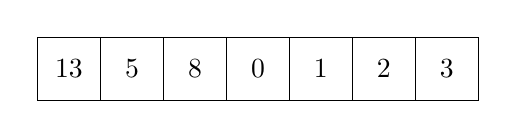
\begin{tikzpicture}
      \matrix (A) [matrix of nodes, nodes={draw, minimum size=8mm},
          column sep=-\pgflinewidth]{
          13 & 5 & 8 & 0 & 1 & 2 & 3\\};
    \end{tikzpicture}
  \end{center}
  \caption{A max heap and its array representation.}
\end{figure}

Heapsort, as you may imagine, utilizes a heap to sort elements. Heapsort
sorts its elements using two routines that 1) build a heap, 2) fix a
heap.

\begin{enumerate}
  \item \textbf{Building a heap.} The first routine is taking the array
    to sort and building a heap from it. This means ordering the array
    elements such that they obey the constraints of a max or min heap.
    For our purposes, the constructed heap will be a \emph{max heap}.
    This means that the largest element, the root of the heap, is the
    first element of the array from which the heap is built.
  \item \textbf{Fixing a heap.} The second routine is needed as we sort
    the array. The gist of Heapsort is that the largest array elements
    are repeatedly removed from the top of the heap and placed at the
    end of the sorted array, if the array is to be sorted in increasing
    order. After removing the largest element from the heap, the heap
    needs to be \emph{fixed} so that it once again obeys the constraints
    of a heap.
\end{enumerate}

In the following Python code for Heapsort, you will notice a lot of
indices are shifted down by 1. Why is this? Recall how indices of
children are computed. The formula of the left child of $k$ being $2k$
only works assuming 1-based indexing. We, in Computer Science,
especially in \textbf{C}, use 0-based indexing. So, we will run the
algorithm assuming 1-based indexing for the Heapsort algorithm itself,
subtracting 1 on each array index access to account for 0-based
indexing.

\begin{pylisting}{Heap maintenance in Python}
def max_child(A: list, first: int, last: int):
    left = 2 * first
    right = left + 1
    if right <= last and A[right - 1] > A[left - 1]:
        return right
    return left

def fix_heap(A: list, first: int, last: int):
    found = False
    mother = first
    great = max_child(A, mother, last)

    while mother <= last // 2 and not found:
        if A[mother - 1] < A[great - 1]:
            A[mother - 1], A[great - 1] = A[great - 1], A[mother - 1]
            mother = great
            great = max_child(A, mother, last)
        else:
            found = True
\end{pylisting}

\begin{pylisting}{Heapsort in Python}
def build_heap(A: list, first: int, last: int):
    for father in range(last // 2, first - 1, -1):
        fix_heap(A, father, last)

def heap_sort(A: list):
    first = 1
    last = len(A)
    build_heap(A, first, last)
    for leaf in range(last, first, -1):
        A[first - 1], A[leaf - 1] = A[leaf - 1], A[first - 1]
        fix_heap(A, first, leaf - 1)
\end{pylisting}

\section{Quicksort}

\epigraph{\emph{If debugging is the process of removing software bugs,
then programming must be the process of putting them in.}}{---Edsger
Dijkstra}

\noindent
Quicksort (sometimes called partition-exchange sort) was developed by
British computer scientist C.A.R. ``Tony'' Hoare in 1959 and published
in 1961. It is perhaps the most commonly used algorithm for sorting (by
competent programmers).  When implemented well, it is the fastest known
algorithm that sorts using \emph{comparisons}. It is usually two or
three times faster than its main competitors, Merge Sort and Heapsort.
It does, though, have a worst case performance of $O(n^2)$ while its
competitors are strictly $O(n \log n)$ in their worst case.

Quicksort is a divide-and-conquer algorithm. It partitions
arrays into two sub-arrays by selecting an element from the array and
designating it as a pivot. Elements in the array that are less than the
pivot go to the left sub-array, and elements in the array that are
greater than or equal to the pivot go to the right sub-array.

Note that Quicksort is an \emph{in-place} algorithm, meaning it doesn't
allocate additional memory for sub-arrays to hold partitioned elements.
Instead, Quicksort utilizes a subroutine called \texttt{partition()}
that places elements less than the pivot into the left side of the array
and elements greater than or equal to the pivot into the right side and
returns the index that indicates the division between the partitioned
parts of the array. Quicksort is then applied recursively on the
partitioned parts of the array, thereby sorting each array partition
containing at least one element. Like with the Heapsort algorithm, the
provided Quicksort pseudocode operates on 1-based indexing, subtracting
one to account for 0-based indexing whenever array elements are
accessed.

\begin{pylisting}{Partition in Python}
def partition(A: list, lo: int, hi: int):
    i = lo - 1
    for j in range(lo, hi):
        if A[j - 1] < A[hi - 1]:
            i += 1
            A[i - 1], A[j - 1] = A[j - 1], A[i - 1]
    A[i], A[hi - 1] = A[hi - 1], A[i]
    return i + 1
\end{pylisting}

\begin{pylisting}{Recursive Quicksort in Python}
# A recursive helper function for Quicksort.
def quick_sorter(A: list, lo: int, hi: int):
    if lo < hi:
        p = partition(A, lo, hi)
        quick_sorter(A, lo, p - 1)
        quick_sorter(A, p + 1, hi)

def quick_sort(A: list):
    quick_sorter(A, 1, len(A))
\end{pylisting}

\section{Batcher's Odd-Even Merge Sort}

\epigraph{\emph{There are two ways of constructing a software design.
    One way is to make it so simple that there are obviously no
    deficiencies, and the other way is to make it so complicated that
    there are no obvious deficiencies. The first method is far more
difficult.}}{---C.A.R. Hoare}

Batcher's odd-even mergesort, or Batcher's method, is unlike the other presented
sorts in that it is actually a \emph{sorting network}. What is a sorting
network? Sorting networks, or \emph{comparator networks}, are circuits built for
the express purpose of sorting a set number of inputs. Sorting networks are
built with a fixed number of wires, one for each input to sort, and are
connected using \emph{comparators}. Comparators compare the values traveling
along the two wires they connect and swap the values if they're out of order.
Since there are a fixed number of comparators, a sorting network must
necessarily sort any input using a fixed number of comparisons. Refer to
Figure~\ref{fig:batcher} for a diagram of a sorting network using Batcher's
method.

Sorting networks are typically limited to inputs that are powers of 2. Batcher's
method is no exception to this. To remedy this, we apply Knuth's modification to
Batcher's method to allow it sort arbitrary-size inputs. This modification on
Batcher's method is also referred to as the \emph{Merge Exchange Sort}. You will
be implementing the merge exchange sort, or Batcher's method, using the
provided Python pseudocode.

\begin{pylisting}{Merge Exchange Sort (Batcher's Method) in Python}
def comparator(A: list, x: int, y: int):
    if A[x] > A[y]:
        A[x], A[y] = A[y], A[x]

def batcher_sort(A: list):
    if len(A) == 0:
        return

    n = len(A)
    t = n.bit_length()
    p = 1 << (t - 1)

    while p > 0:
        q = 1 << (t - 1)
        r = 0
        d = p

        while d > 0:
            for i in range(0, n - d):
                if (i & p) == r:
                    comparator(A, i, i + d)
            d = q - p
            q >>= 1
            r = p

        p >>= 1
\end{pylisting}

The pseudocode for Batcher's method can be a little mysterious, but it
effectively acts as a parallel \emph{Shell Sort}. Shell Sort acts a variation of
Insert Sort and first sorts pairs of elements which are far apart from each
other. The distance between these pairs of elements is called a \emph{gap}. Each
iteration of Shell Sort decreases the gap until a gap of $1$ is used.

Batcher's method is similar, but instead of sorting pairs of elements that are a
set gap apart, it \emph{$k$-sorts} the even and odd subsequences of the array,
where $k$ is some power of $2$. Given an array $A$ where $A_i$ denotes the
$i$-th index of $A$, an even subsequence refers to the sequence of values
$\{A_0, A_2, A_4, \dots \}$. Similarly, an odd subsequence refers to the sequence
of values $\{A_1, A_3, A_5, \dots \}$. The topic of $k$-sorting is beyond the
scope of this course, but all that you are required to understand is that if an
array is $k$-sorted, then all its elements are at most $k$ indices away from its
sorted position.

Consider an array of $16$ elements. Batcher's method first $8$-sorts the even
and odd subsequences, then $4$-sorts them, then $2$-sorts them, and finally
$1$-sorts them, \emph{merging} the sorted even and odd sequences. We will call
each level of $k$-sorting a \emph{round}. As stated previously, Batcher's method
works in \emph{parallel}. By virtue of the algorithm, any indices that appear in
a pairwise comparison when $k$-sorting a subsequence do not appear as indices in
another comparison during the same round. A clever use of the bitwise AND
operator, \texttt{\&}, guarantees this property.

When computing the bitwise AND operator of two integers $x$ and $y$, the
resulting integer is composed of $0$-bits except in the positions where both $x$
and $y$ have a $1$-bit. As an example, let $x = 10 = 1010_2$ and $y = 8 =
1000_2$. Bitwise AND-ing $x$ and $y$ yields $z = 8 = 1000_2$. In the provided
pseudocode, the variable \texttt{p} tracks the current round of $k$-sorting. It
is always a power of 2 since it starts off as a power of 2, and is only halved
in value using the right-shift operator (\verb|>>|). The condition on line 20 of
the pseudocode first computes the bitwise AND of \texttt{i} and \texttt{p}. This
effectively partitions values of \texttt{i} into partitions of size \texttt{p}.
The variable \texttt{r} effectively represents which partitions can be
considered for comparison. Thus, \texttt{(i \& p) == r} checks if the partition
that \texttt{i} falls into is eligible for comparison, and if it is, to execute
the comparison.

Indices are only ever compared with indices that are \texttt{d} indices away.
Since \texttt{p} is a power of $2$ and \texttt{d} is an odd multiple of
\texttt{p}, it follows that \texttt{i \& p != (i + d) \& p} for any \texttt{i}.
This means there is no overlap with any of the pairs of indices, which therefore
means that these comparisons can be run simultaneously, or in \emph{parallel},
with no ill effect. These parallel comparisons are shown clearly in
Figure~\ref{fig:batcher}.

Although Batcher's method can be run in parallel, your implementation of the
sort will run \emph{sequentially}, sorting the input over several rounds. For an
array size of $n$, the initial value to $k$-sort with is $k = \lceil \log_2(n)
\rceil$. The even and odd subsequences are first $k$-sorted, then
$\frac{k}{2}$-sorted, then $\frac{k}{4}$-sorted, and so on until they are
$1$-sorted. You will want to edit the provided pseudocode to print out the pairs
of indices that are being compared to see what is happening.

\begin{figure}[htb]
  \centering
  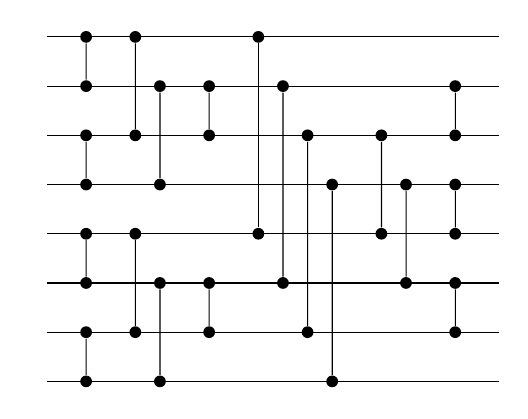
\begin{tikzpicture}[>=latex',scale=1.25]
    % Wire 0 line.
    \node at (0,-1.0) (wire0) {};
    \draw[-] (wire0.east) -- +(4.6,0);
    \node at (0.5,-1.0) (c01) [circle,fill,inner sep=1.5pt]{};
    \node at (1.0,-1.0) (c02) [circle,fill,inner sep=1.5pt]{};
    \node at (2.25,-1.0) (c03) [circle,fill,inner sep=1.5pt]{};

    % Wire 1 line.
    \node at (0,-1.5) (wire1) {};
    \draw[-] (wire1.east) -- +(4.6,0);
    \node at (0.5,-1.5) (c11) [circle,fill,inner sep=1.5pt]{};
    \node at (1.25,-1.5) (c12) [circle,fill,inner sep=1.5pt]{};
    \node at (1.75,-1.5) (c13) [circle,fill,inner sep=1.5pt]{};
    \node at (2.5,-1.5) (c14) [circle,fill,inner sep=1.5pt]{};
    \node at (4.25,-1.5) (c15) [circle,fill,inner sep=1.5pt]{};

    % Wire 2 line.
    \node at (0,-2.0) (wire2) {};
    \draw[-] (wire2.east) -- +(4.6,0);
    \node at (0.5,-2.0) (c21) [circle,fill,inner sep=1.5pt]{};
    \node at (1.0,-2.0) (c22) [circle,fill,inner sep=1.5pt]{};
    \node at (1.75,-2.0) (c23) [circle,fill,inner sep=1.5pt]{};
    \node at (2.75,-2.0) (c24) [circle,fill,inner sep=1.5pt]{};
    \node at (3.5,-2.0) (c25) [circle,fill,inner sep=1.5pt]{};
    \node at (4.25,-2.0) (c26) [circle,fill,inner sep=1.5pt]{};

    % Wire 3 line.
    \node at (0,-2.5) (wire3) {};
    \draw[-] (wire3.east) -- +(4.6,0);
    \node at (0.5,-2.5) (c31) [circle,fill,inner sep=1.5pt]{};
    \node at (1.25,-2.5) (c32) [circle,fill,inner sep=1.5pt]{};
    \node at (3.0,-2.5) (c33) [circle,fill,inner sep=1.5pt]{};
    \node at (3.75,-2.5) (c34) [circle,fill,inner sep=1.5pt]{};
    \node at (4.25,-2.5) (c35) [circle,fill,inner sep=1.5pt]{};

    % Wire 4 line.
    \node at (0,-3.0) (wire4) {};
    \draw[-] (wire4.east) -- +(4.6,0);
    \node at (0.5,-3.0) (c41) [circle,fill,inner sep=1.5pt]{};
    \node at (1.0,-3.0) (c42) [circle,fill,inner sep=1.5pt]{};
    \node at (2.25,-3.0) (c43) [circle,fill,inner sep=1.5pt]{};
    \node at (3.5,-3.0) (c44) [circle,fill,inner sep=1.5pt]{};
    \node at (4.25,-3.0) (c45) [circle,fill,inner sep=1.5pt]{};

    % Wire 5 line.
    \node at (0,-3.5) (wire5) {};
    \draw[-] (wire5.east) -- +(4.6,0);
    \node at (0.5,-3.5) (c51) [circle,fill,inner sep=1.5pt]{};
    \node at (1.25,-3.5) (c52) [circle,fill,inner sep=1.5pt]{};
    \node at (1.75,-3.5) (c53) [circle,fill,inner sep=1.5pt]{};
    \node at (2.5,-3.5) (c54) [circle,fill,inner sep=1.5pt]{};
    \node at (3.75,-3.5) (c55) [circle,fill,inner sep=1.5pt]{};
    \node at (4.25,-3.5) (c56) [circle,fill,inner sep=1.5pt]{};

    % Wire 6 line.
    \node at (0,-4.0) (wire6) {};
    \draw[-] (wire6.east) -- +(4.6,0);
    \node at (0.5,-4.0) (c61) [circle,fill,inner sep=1.5pt]{};
    \node at (1.0,-4.0) (c62) [circle,fill,inner sep=1.5pt]{};
    \node at (1.75,-4.0) (c63) [circle,fill,inner sep=1.5pt]{};
    \node at (2.75,-4.0) (c64) [circle,fill,inner sep=1.5pt]{};
    \node at (4.25,-4.0) (c65) [circle,fill,inner sep=1.5pt]{};

    % Wire 7 line.
    \node at (0,-4.5) (wire7) {};
    \draw[-] (wire7.east) -- +(4.6,0);
    \node at (0.5,-4.5) (c71) [circle,fill,inner sep=1.5pt]{};
    \node at (1.25,-4.5) (c72) [circle,fill,inner sep=1.5pt]{};
    \node at (3.0,-4.5) (c73) [circle,fill,inner sep=1.5pt]{};

    % Comparators.
    \draw[-] (c01) -- (c11);
    \draw[-] (c21) -- (c31);
    \draw[-] (c41) -- (c51);
    \draw[-] (c61) -- (c71);
    \draw[-] (c02) -- (c22);
    \draw[-] (c42) -- (c62);
    \draw[-] (c12) -- (c32);
    \draw[-] (c52) -- (c72);
    \draw[-] (c13) -- (c23);
    \draw[-] (c53) -- (c63);
    \draw[-] (c03) -- (c43);
    \draw[-] (c14) -- (c54);
    \draw[-] (c24) -- (c64);
    \draw[-] (c33) -- (c73);
    \draw[-] (c25) -- (c44);
    \draw[-] (c34) -- (c55);
    \draw[-] (c15) -- (c26);
    \draw[-] (c35) -- (c45);
    \draw[-] (c56) -- (c65);
  \end{tikzpicture}
  \caption{
    Batcher's odd-even mergesort sorting network with eight inputs. Inputs
    traveling along the wires are sorted as they move from left to right.
}
  \label{fig:batcher}
\end{figure}

\section{Your Task}

\epigraphwidth=0.5\textwidth
\epigraph{\emph{The people will believe what the media tells them they
believe.}}{---George Orwell}

\noindent
\begin{itemize}
  \item Initialize your Bloom filter and hash table.
  \item Read in a list of \emph{badspeak} words with \texttt{fscanf()}.
    Again, badspeak is simply oldspeak without a newspeak translation.
    Badspeak is strictly forbidden. Each badspeak word should be added
    to the Bloom filter and the hash table. The list of proscribed words
    will be in \texttt{badspeak.txt}, which can be found in the
    \texttt{resources} repository.
  \item Read in a list of \emph{oldspeak} and \emph{newspeak} pairs with
    \texttt{fscanf()}. Only the oldspeak should be added to the Bloom
    filter. The oldspeak \emph{and} newspeak are added to the hash
    table. The list of oldspeak and newspeak pairs will be in
    \texttt{newspeak.txt}, which can also be found in the
    \texttt{resources} repository.
  \item Now that the lexicon of badspeak and oldspeak/newspeak
    translations has been populated, you can start to filter out words.
    Read words in from \texttt{stdin} using the supplied parsing module.
  \item For each word that is read in, check to see if it has been added
    to the Bloom filter. If it has not been added to the Bloom filter,
    then no action is needed since the word isn't a proscribed word.
  \item If the word has most likely been added to the Bloom filter,
    meaning \texttt{bf\_probe()} returned \texttt{true}, then further
    action needs to be taken.
    \begin{enumerate}
      \item If the hash table contains the word and the word \emph{does
        not} have a newspeak translation, then the citizen who used this
        word is guilty of \texttt{thoughtcrime}. Insert this badspeak
        word into a list of badspeak words that the citizen used in
        order to notify them of their errors later. What data structure
        could be used to store these words?
      \item If the hash table contains the word, and the word \emph{does}
        have a newspeak translation, then the citizen requires
        counseling on proper \emph{Rightspeak}. Insert this oldspeak
        word into a list of oldspeak words with newspeak translations in
        order to notify the citizen of the revisions needed to be made
        in order to practice Rightspeak.
      \item If the hash table does not contain the word, then all is
        good since the Bloom filter issued a false positive. No
        disciplinary action needs to be taken.
    \end{enumerate}
  \item If the citizen is accused of thoughtcrime \emph{and} requires
    counseling on proper \emph{Rightspeak}, then they are given a
    reprimanding \emph{mixspeak message} notifying them of their
    transgressions and promptly sent off to \emph{joycamp}. The message
    should contain the list of badspeak words that were used followed by
    the list of oldspeak words that were used with their proper newspeak
    translations.

  \begin{shlisting}{}
Dear beloved citizen of the GPRSC,

We have some good news, and we have some bad news.
The good news is that there is bad news. The bad news is that you will
be sent to joycamp and subjected to a week-long destitute existence.
This is the penalty for using degenerate words, as well as using
oldspeak in place of newspeak. We hope you can correct your behavior.

Your transgressions, followed by the words you must think on:

kalamazoo
antidisestablishmentarianism
write -> papertalk
sad -> happy
read -> papertalk
music -> noise
liberty -> badfree\end{shlisting}

  \item If the citizen is accused solely of thoughtcrime, then they are
    issued a thoughtcrime message and also sent off to \emph{joycamp}.
    The \emph{badspeak message} should contain the list of badspeak
    words that were used.

  \begin{shlisting}{}
Dear beloved citizen of the GPRSC,

You have been caught using degenerate words that may cause
distress among the moral and upstanding citizens of the GPSRC.
As such, you will be sent to joycamp. It is there where you will
sit and reflect on the consequences of your choice in language.

Your transgressions:

kalamazoo
antidisestablishmentarianism\end{shlisting}

  \item If the citizen only requires counseling, then they are issued an
    encouraging \emph{goodspeak message}. They will read it, correct
    their \emph{wrongthink}, and enjoy the rest of their stay in the
    GPRSC. The message should contain the list of oldspeak words that
    were used with their proper newspeak translations.

    \begin{shlisting}{}
Dear beloved citizen of the GPRSC,

We recognize your efforts in conforming to the language standards
of the GPSRC. Alas, you have been caught uttering questionable words
and thinking unpleasant thoughts. You must correct your wrongspeak
and badthink at once. Failure to do so will result in your deliverance
to joycamp.

Words that you must think on:

write -> papertalk
sad -> happy
read -> papertalk
music -> noise
liberty -> badfree\end{shlisting}

  \item Each of the messages are defined for you in \texttt{messages.h}.
    \textcolor{red}{You may not modify this file}.

  \item The list of the command-line options your program must support
    is listed below. \emph{Any} combination of the command-line options
    must be supported.
    \begin{itemize}
      \item \texttt{-h} prints out the program usage. Refer to the
      reference program in the resources repository for what to print.
      \item \texttt{-t size} specifies that the hash table
        will have \texttt{size} entries (the default will be $2^{16}$).
      \item \texttt{-f size} specifies that the Bloom filter
        will have \texttt{size} entries (the default will be $2^{20}$).
      \item \texttt{-s} will enable the printing of statistics to
        \texttt{stdout}. The statistics to calculate are:
        \begin{itemize}
          \item Average binary search tree size
          \item Average binary search tree height
          \item Average branches traversed
          \item Hash table load
          \item Bloom filter load
        \end{itemize}
        The latter three statistics are computed as follows:
        \begin{align*}
          \text{Average branches traversed} &=
          \frac{\texttt{branches}}{\texttt{lookups}} \\
          \text{Hash table load} &= 100 \times \frac{\texttt{ht\_count()}}{\texttt{ht\_size()}} \\
          \text{Bloom filter load} &= 100 \times \frac{\texttt{bf\_count()}}{\texttt{bf\_size()}}
        \end{align*}
        The hash table load and Bloom filter load should be printed with
        up to 6 digits of precision. \textcolor{red}{Enabling the
        printing of statistics should \emph{suppress all messages} the
        program may otherwise print.} The number of lookups is defined
        as the number of times \texttt{ht\_lookup()} and
        \texttt{ht\_insert()} is called. The number of branches is
        defined as the count of links traversed during calls to
        \texttt{bst\_find()} and \texttt{bst\_insert()}. The global
        variable \texttt{lookups} should be defined in \texttt{ht.c} and
        the global variable \texttt{branches} should be defined in
        \texttt{bst.c}.
    \end{itemize}
\end{itemize}

\section{Sets}

For this assignment, you are required to use a \emph{set} to track which
command-line options are specified when your program is run. The code
for sets is given in the resources repository in \texttt{set.h}.
\textcolor{red}{You may not modify this file.} Make sure to take the
time to go through and understand the code.

For manipulating the bits in a set, we use bit-wise operators. These
operators, as the name suggests, will perform an operation on every bit
in a number. The following are the six bit-wise operators specified in
\textbf{C}:

\begin{center}
  \begin{tabular}{|c|l|l|}
    \hline
    \verb|&| & bit-wise AND & Performs the AND operation on every bit
    of two numbers. \\
    \hline
    \verb||| & bit-wise OR & Performs the OR operation on every bit of
    two numbers. \\
    \hline
    \verb|~| & bit-wise NOT & Inverts all bits in the given number. \\
    \hline
    \verb|^| & bit-wise XOR & Performs the exclusive-OR operation on
    every bit of two numbers. \\
    \hline
    \verb|<<| & left shift & Shifts bits in a number to the left by a
    specified number of bits. \\
    \hline
    \verb|>>| & right shift & Shifts bits in a number to the right by a
    specified number of bits. \\
    \hline
  \end{tabular}
\end{center}

\noindent Recall that the basic set operations are: \emph{membership},
\emph{union}, \emph{intersection} and \emph{negation}. The functions
implementing these set operations are implemented for you. Using these
functions, you will set (make the bit 1) or clear (make the bit 0) bits
in the \texttt{Set} depending on the command-line options read by
\texttt{getopt()}. You can then check the states of all the bits (the
members) of the \texttt{Set} using a single \texttt{for} loop and
execute the corresponding sort. Note: you most likely won't use all the
functions, but you \emph{must} use sets to track which command-line
options are specified when running your program.

\begin{funcdoc}{\texttt{Set empty\_set(void)}}
  This function is used to return an empty set. In this context, an empty
  set would be a set in which all bits are equal to 0.
\end{funcdoc}

\begin{funcdoc}{\texttt{bool member\_set(uint32\_t x, Set s)}}

\begin{align*}
  x \in s \iff x\, \text{is a member of set}\, s
\end{align*}

  \noindent This function returns a \texttt{bool} indicating the
  presence of the given value \texttt{x} in the set \texttt{s}. The
  bit-wise AND operator is used to determine set membership. The first
  operand for the AND operation is the set \texttt{s}. The second
  operand is the value obtained by left shifting 1 \texttt{x} number of
  times. If the result of the AND operation is a non-zero value, then
  \texttt{x} is a member of \texttt{s} and \texttt{true} is returned to
  indicate this. \texttt{false} is returned if the result of the AND
  operation is 0.
\end{funcdoc}

\begin{funcdoc}{\texttt{Set insert\_set(uint32\_t x, Set s)}}
  This function inserts \texttt{x} into \texttt{s}. That is, it returns
  set \texttt{s} with the bit corresponding to \texttt{x} set to 1.
  Here, the bit is set using the bit-wise OR operator. The first operand
  for the OR operation is the set \texttt{s}. The second operand is
  value obtained by left shifting 1 by \texttt{x} number of bits.
\end{funcdoc}

\begin{funcdoc}{\texttt{Set delete\_set(uint32\_t x, Set s)}}
  This function deletes (removes) \texttt{x} from \texttt{s}. That is,
  it returns set \texttt{s} with the bit corresponding to \texttt{x}
  cleared to 0. Here, the bit is cleared using the bit-wise AND
  operator. The first operand for the AND operation is the set
  \texttt{s}. The second operand is a negation of the number 1 left
  shifted to the same position that \texttt{x} would occupy in the set.
  This means that the bits of the second operand are all 1s except for
  the bit at \texttt{x}'s position. The function returns set \texttt{s}
  after removing \texttt{x}.
\end{funcdoc}

\begin{funcdoc}{\texttt{Set union\_set(Set s, Set t)}}

\begin{align*}
  s \cup t = \{x | x \in s \lor x \in  t\}
\end{align*}

  \noindent The union of two sets is a collection of all elements in
  both sets. Here, to calculate the union of the two sets \texttt{s} and
  \texttt{t}, we need to use the OR operator. Only the bits
  corresponding to members that are equal to 1 in either \texttt{s} or
  \texttt{t} are in the new set returned by the function.
\end{funcdoc}

\begin{funcdoc}{\texttt{Set intersect\_set(Set s, Set t)}}

\begin{align*}
  s \cap t = \{x | x \in s \land x \in  t\}
\end{align*}

  \noindent The intersection of two sets is a collection of elements that
  are common to both sets. Here, to calculate the intersection of the
  two sets \texttt{s} and \texttt{t}, we need to use the AND operator.
  Only the bits corresponding to members that are equal to 1 in both
  \texttt{s} and \texttt{t} are in the new set returned by the function.
\end{funcdoc}

\begin{funcdoc}{\texttt{Set difference\_set(Set s, Set t)}}
  The difference of two sets refers to the elements of set \texttt{s}
  which are not in set \texttt{t}. In other words, it refers to the
  members of set \texttt{s} that are unique to set \texttt{s}. The
  difference is calculated using the AND operator where the two operands
  are set \texttt{s} and the negation of set \texttt{t}. The function
  then returns the set of elements in \texttt{s} that are not in
  \texttt{t}.

  This function can be used to find the complement of a given set as well,
  in which case the first operand would be the universal set $\mathbb{U}$
  and the second operand would be the set you want to complement as shown
  below.
\end{funcdoc}

\begin{align*}
  \overline{s} = \{ x | x \notin s\} = \mathbb{U} -s
\end{align*}

\begin{funcdoc}{\texttt{Set complement\_set(Set s)}}
  This function is used to return the complement of a given set. By
  complement we mean that all bits in the set are flipped using the NOT
  operator. Thus, the set that is returned contains all the elements of
  the universal set $\mathbb{U}$ that are not in \texttt{s} and contains
  none of the elements that are present in \texttt{s}.
\end{funcdoc}

\section{Testing}

\begin{itemize}
  \item You will test each of the sorts specified by command-line option
    by sorting an array of pseudorandom numbers generated with
    \texttt{random()}. Each of your sorts should sort the \emph{same}
    pseudorandom array. \textcolor{red}{Hint: make use of
    \texttt{srandom()}.}
  \item The pseudorandom numbers generated by \texttt{random()} should
    be \emph{bit-masked} to fit in \emph{30} bits. \textcolor{red}{Hint: use
    bit-wise AND.}
  \item Your test harness \emph{must} be able to test your sorts with
    array sizes \emph{up to the memory limit of the computer}. That
    means that you will need to dynamically allocate the array.
  \item Your program should have no \emph{memory leaks}. Make sure you
    \texttt{free()} before exiting. \texttt{valgrind} should pass
    cleanly with any combination of the specified command-line options.
  \item Your algorithms \emph{must} correctly sort. Any algorithm that
    does not sort correctly will receive a \emph{zero}.
\end{itemize}

A large part of this assignment is understanding and comparing the
performance of various sorting algorithms. You essentially conducting an
experiment. As stated in \S\ref{task}, you \emph{must} collect the following
statistics on each algorithm:

\begin{itemize}
  \item The \emph{size} of the array,
  \item The number of \emph{moves} required (each time you transfer an
    element in the array, that counts), and
  \item The number of \emph{comparisons} required (comparisons
    \emph{only} count for \emph{elements}, not for logic).
\end{itemize}

\section{Output}
\epigraph{\emph{Books are not made to be believed, but to be subjected to inquiry. When we consider a book, we mustn’t ask ourselves what it says but what it means.}}{---Umberto Eco}

\noindent
The output your test harness produces \emph{must} be formatted like in
the following examples:

\begin{shlisting}{}
$ ./sorting -q -n 1000 -p 0
Quick Sort, 1000 elements, 18642 moves, 10531 compares
$ ./sorting -h -n 15 -p 0
Heap Sort, 15 elements, 144 moves, 70 compares
$ ./sorting -a -n 15
Shell Sort, 15 elements, 90 moves, 59 compares
     34732749     42067670     54998264    102476060    104268822
    134750049    182960600    538219612    629948093    783585680
    954916333    966879077    989854347    994582085   1072766566
Batcher Sort, 15 elements, 90 moves, 59 compares
     34732749     42067670     54998264    102476060    104268822
    134750049    182960600    538219612    629948093    783585680
    954916333    966879077    989854347    994582085   1072766566
Heap Sort, 15 elements, 144 moves, 70 compares
     34732749     42067670     54998264    102476060    104268822
    134750049    182960600    538219612    629948093    783585680
    954916333    966879077    989854347    994582085   1072766566
Quick Sort, 15 elements, 135 moves, 51 compares
     34732749     42067670     54998264    102476060    104268822
    134750049    182960600    538219612    629948093    783585680
    954916333    966879077    989854347    994582085   1072766566
\end{shlisting}

For each sort that was specified, print its name, the statistics for the
run, then the specified number of array elements to print. The array
elements should be printed out in a table with 5 columns. Each array
element should be printed with a width of 13. You should make use of the
following \texttt{printf()} statement:

\begin{clisting}{}
printf("%13" PRIu32); // Include <inttypes.h> for PRIu32.
\end{clisting}

\section{Statistics}
\epigraph{\emph{There are three types of lies---lies, damn lies, and statistics.}}{%
---Benjamin Disraeli}

\noindent
To facilitate the gathering of statistics, you will be given,
\textcolor{red}{\emph{and must use}}, a small statistics module. The
module itself revolves around the following struct:

\begin{clisting}{}
typedef struct {
  uint64_t moves;
  uint64_t comparisons;
} Stats;
\end{clisting}

The module also includes functions to \emph{compare}, \emph{swap}, and
\emph{move} elements.

\begin{funcdoc}{int cmp(Stats *stats, uint32\_t x, uint32\_t y)}
  Compares \texttt{x} and \texttt{y} and increments the
  \texttt{comparisons} field in \texttt{stats}. Returns \texttt{-1} if
  \texttt{x} is less than \texttt{y}, \texttt{0} if \texttt{x} is equal
  to \texttt{y}, and \texttt{1} if \texttt{x} is greater than
  \texttt{y}.
\end{funcdoc}

\begin{funcdoc}{uint32\_t move(Stats *stats, uint32\_t x)}
  ``Moves'' \texttt{x} by incrementing the \texttt{moves} field in
  \texttt{stats} and returning \texttt{x}. This is intended for use in
  Insertion Sort and Shell Sort, where array elements aren't swapped,
  but instead moved and stored in a temporary variable.
\end{funcdoc}

\begin{funcdoc}{void swap(Stats *stats, uint32\_t *x, uint32\_t *y)}
  Swaps the elements pointed to by pointers \texttt{x} and \texttt{y},
  incrementing the \texttt{moves} field in \texttt{stats} by 3 to
  reflect a swap using a temporary variable.
\end{funcdoc}

\begin{funcdoc}{void reset(Stats *stats)}
  Resets \texttt{stats}, setting the \texttt{moves} field and
  \texttt{comparisons} field to 0. It is possible that you don't end up
  using this specific function, depending on your usage of the
  \texttt{Stats} \texttt{struct}.
\end{funcdoc}

\section{Deliverables}

\epigraphwidth=0.4\textwidth
\epigraph{\emph{It is such a sweet temptation \\ It gives such grief relief \\
It is such a false sensation \\ How come that's so hard to believe?}}{---Ray
Wylie Hubbard, \emph{Loco Gringo's Lament}}

You will need to turn in the following source code and header files:

\begin{enumerate}
  \item Your program \emph{must} have the following source and header
    files:
  \begin{itemize}
    \item \texttt{universe.c} implements the \texttt{Universe} ADT.
    \item \texttt{universe.h} specifies the interface to the \texttt{Universe}
      ADT. This file is provided and \emph{may not} be modified.
    \item \texttt{life.c} contains \texttt{main()} and \emph{may}
      contain any other functions necessary to complete your implementation of
      the Game of Life.
  \end{itemize}
\end{enumerate}

You can have other source and header files, but \emph{do not try to be overly
clever}. You will also need to turn in the following:

\begin{enumerate}
  \item \texttt{Makefile}:
    \begin{itemize}
      \item \texttt{CC = clang} must be specified.
      \item \texttt{CFLAGS = -Wall -Wextra -Werror -Wpedantic} must be specified.
      \item \texttt{make} must build the \texttt{life} executable, as should
        \texttt{make all} and \texttt{make life}.
      \item \texttt{make clean} must remove all files that are compiler
        generated.
      \item \texttt{make format} should format all your source code,
        including the header files.
    \end{itemize}
  \item \texttt{README.md}: This must use proper Markdown syntax. It
    must describe how to use your program and \texttt{Makefile}. It
    should also list and explain any command-line options that your
    program accepts. Any false positives reported by \texttt{scan-build}
    should be documented and explained here as well. Note down any known
    bugs or errors in this file as well for the graders.
  \item \texttt{DESIGN.pdf}: This document \emph{must} be a proper
    PDF\@. This design document must describe your design and design
    process for your program with enough detail such that a sufficiently
    knowledgeable programmer would be able to replicate your
    implementation. \textcolor{red}{This does not mean copying your
    entire program in verbatim}. You should instead describe how your
    program works with supporting pseudocode.
  \item \texttt{WRITEUP.pdf}: This document \emph{must} be a proper
    PDF\@. This writeup document must include everything you learned from
    this assignment. Make sure to mention everything in detail while being as precise as possible. How well you explain all the lessons you have learned in this assignment will be really important here. 
\end{enumerate}

\section{Submission}

Refer back assignment 0 for the instructions on how to properly submit
your assignment through \texttt{git}. Remember: \emph{add},
\emph{commit}, and \emph{push}!

\textcolor{red}{Your assignment is turned in \emph{only} after you have
pushed and submitted the commit ID you want graded on Canvas. ``I
forgot to push'' and ``I forgot to submit my commit ID'' are not valid
excuses. It is \emph{highly} recommended to commit and push your changes
\emph{often}.}

\section{Supplemental Readings}

\epigraph{\emph{The more that you read, the more things you will know. The
more that you learn, the more places you'll go.}}{---Dr.\ Seuss}

\begin{itemize}
  \item \textit{The C Programming Language} by Kernighan \& Ritchie
  \begin{itemize}
    \item Chapter 7
    \item Appendix B
  \end{itemize}
  \item \textit{Introduction to Algorithms} by T.\ Cormen, C.\
    Leiserson, R.\ Rivest, \& C.\ Stein
    \begin{itemize}
      \item Chapter 31 \S 31.2, \S 31.3, \S 31.6, \S 31.7, \S 31.8
    \end{itemize}
\end{itemize}


\monkey{Paggimmnorr in C is eikl ggiinv a ekmnoy a aachinsw.}

\end{document}
